\documentclass[a4paper, 14pt]{article}				% general format

\usepackage[utf8]{inputenc}					% accept different input encodings
\usepackage[russian]{babel}					% multilingual support (T2A)
\usepackage{graphicx}
\usepackage{float}
\usepackage{amsmath}
\usepackage[boxed]{algorithm2e}
\usepackage{url}
\usepackage{fancyvrb}
\usepackage[dvipsnames]{xcolor}

\usepackage{listings}						% typeset source code listings

% Цвета для кода
\definecolor{string}{HTML}{101AF9}			% цвет строк в коде
\definecolor{comment}{HTML}{3F7F5F}		% цвет комментариев в коде
\definecolor{keyword}{HTML}{5F1441}			% цвет ключевых слов в коде
\definecolor{morecomment}{HTML}{8000FF}		% цвет include и других элементов в коде
\definecolor{captiontext}{HTML}{FFFFFF}		% цвет текста заголовка в коде
\definecolor{captionbk}{HTML}{999999}		% цвет фона заголовка в коде
\definecolor{bk}{HTML}{FFFFFF}			% цвет фона в коде
\definecolor{frame}{HTML}{999999}			% цвет рамки в коде

% Настройки отображения кода
\lstset{
	language=C++,						% Язык кода по умолчанию
	% Цвета
	keywordstyle=\color{keyword}\ttfamily\bfseries,
	stringstyle=\color{string}\ttfamily,
	commentstyle=\color{comment}\ttfamily\itshape,
	morecomment=[l][\color{morecomment}]{\#},
	% Настройки отображения
	breaklines=true,					% Перенос длинных строк
	basicstyle=\ttfamily\footnotesize,		% Шрифт для отображения кода
	backgroundcolor=\color{bk},			% Цвет фона кода
	frame=tblr						% draw a frame at all sides of the code block
	rulecolor=\color{frame},				% Цвет рамки
	tabsize=2,						% tab space width
	showstringspaces=false,				% don't mark spaces in strings
	% Настройка отображения номеров строк. Если не нужно, то удалите весь блок
	numbers=left,					% Слева отображаются номера строк
	stepnumber=1,					% Каждую строку нумеровать
	numbersep=5pt,					% Отступ от кода
	numberstyle=\small\color{black},			% Стиль написания номеров строк
	}
% Для настройки заголовка кода
\usepackage{caption}
\DeclareCaptionFont{white}{\color{сaptiontext}}
\DeclareCaptionFormat{listing}{\parbox{\linewidth}{\colorbox{сaptionbk}{\parbox{\linewidth}{#1#2#3}}\vskip-4pt}}
%\captionsetup[lstlisting]{format=listing,labelfont=white,textfont=white}
\renewcommand{\lstlistingname}{Листинг} % Переименование Listings в нужное именование структуры

\author{Певцов Игорь, гр.53501/3}
\title{Отчет по лабораторной работе 4:\\"Утилита для исследования сети и сканер портов Nmap"\\ по дисциплине\\"Методы и средства защиты информации"}

\begin{document}
\maketitle

\newpage
\tableofcontents{}

\newpage
\section{Утилита для исследования сети и сканер портов Nmap.}

\subsection{Цель работы}
Изучение принципов работы утилиты Nmap на примере локальной сети
\subsection{Ход работы}

Работа выполнялась в домашней локальной сети с адресами 192.168.1.0/24, а также в сети VMware 192.168.32.0/24

\subsubsection{Определение набора и версии сервисов, запущенных на компьютере в диапазоне адресов.}
\paragraph{Сканирование хостов\\}

Проводим поиск активных хостов. Для этого необходимо ввести команду
\begin{Verbatim}[frame=single]
	nmap -sn 192.168.1.0-254
\end{Verbatim}
Ключ -sn служит для ''быстрого'' сканирования, когда не сканируются порты.
Результат выполнения команды:
\begin{figure}[h!]
\centering
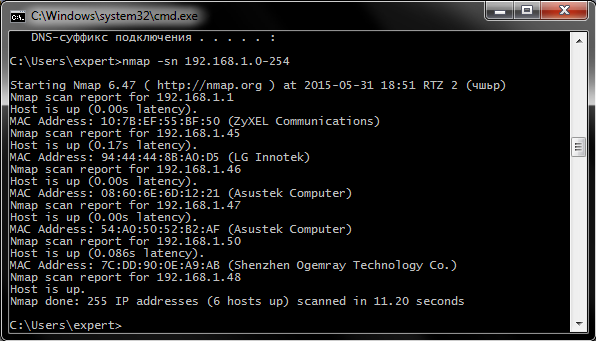
\includegraphics[width=\textwidth]{rsrc/nmap_1}
\caption{Сканирование хостов.}
\end{figure}

\newpage
\paragraph{Сканирование портов\\}
Чтобы просканировать порты используем команду

\begin{Verbatim}[frame=single]
	nmap --top-ports 10 192.168.1.0-254
\end{Verbatim}

Ключ --top-ports 10 используется для вывода информации о 10 наиболее активных портах в заданном диапазоне адресов.
Результат выполнения команды:
\begin{Verbatim}[frame=single]
Starting Nmap 6.47 ( http://nmap.org ) at 2015-05-31 18:56 RTZ 2
Nmap scan report for 192.168.1.1
Host is up (0.0074s latency).
PORT     STATE  SERVICE
21/tcp   closed ftp
22/tcp   closed ssh
23/tcp   open   telnet
25/tcp   closed smtp
80/tcp   open   http
110/tcp  closed pop3
139/tcp  open   netbios-ssn
443/tcp  closed https
445/tcp  open   microsoft-ds
3389/tcp closed ms-wbt-server
MAC Address: 10:7B:EF:55:BF:50 (ZyXEL Communications)

Nmap scan report for 192.168.1.43
Host is up (0.12s latency).
PORT     STATE    SERVICE
21/tcp   filtered ftp
22/tcp   filtered ssh
23/tcp   filtered telnet
25/tcp   filtered smtp
80/tcp   filtered http
110/tcp  filtered pop3
139/tcp  filtered netbios-ssn
443/tcp  filtered https
445/tcp  filtered microsoft-ds
3389/tcp filtered ms-wbt-server
MAC Address: 04:DB:56:2D:82:76 (Apple)

Nmap scan report for 192.168.1.45
Host is up (0.028s latency).
PORT     STATE  SERVICE
21/tcp   closed ftp
22/tcp   closed ssh
23/tcp   closed telnet
25/tcp   closed smtp
80/tcp   closed http
110/tcp  closed pop3
139/tcp  closed netbios-ssn
443/tcp  closed https
445/tcp  closed microsoft-ds
3389/tcp closed ms-wbt-server
MAC Address: 94:44:44:8B:A0:D5 (LG Innotek)

Nmap scan report for 192.168.1.46
Host is up (0.0040s latency).
PORT     STATE    SERVICE
21/tcp   filtered ftp
22/tcp   filtered ssh
23/tcp   filtered telnet
25/tcp   filtered smtp
80/tcp   open     http
110/tcp  filtered pop3
139/tcp  filtered netbios-ssn
443/tcp  open     https
445/tcp  filtered microsoft-ds
3389/tcp filtered ms-wbt-server
MAC Address: 08:60:6E:6D:12:21 (Asustek Computer)

Nmap scan report for 192.168.1.47
Host is up (0.0032s latency).
PORT     STATE    SERVICE
21/tcp   filtered ftp
22/tcp   filtered ssh
23/tcp   filtered telnet
25/tcp   filtered smtp
80/tcp   filtered http
110/tcp  filtered pop3
139/tcp  open     netbios-ssn
443/tcp  filtered https
445/tcp  open     microsoft-ds
3389/tcp filtered ms-wbt-server
MAC Address: 54:A0:50:52:B2:AF (Asustek Computer)

Nmap scan report for 192.168.1.50
Host is up (0.026s latency).
PORT     STATE  SERVICE
21/tcp   open   ftp
22/tcp   open   ssh
23/tcp   open   telnet
25/tcp   closed smtp
80/tcp   open   http
110/tcp  closed pop3
139/tcp  open   netbios-ssn
443/tcp  closed https
445/tcp  closed microsoft-ds
3389/tcp closed ms-wbt-server
MAC Address: 7C:DD:90:0E:A9:AB (Shenzhen Ogemray Technology Co.)

Skipping SYN Stealth Scan against 192.168.1.48 because Windows does not support
scanning your own machine (localhost) this way.
Nmap scan report for 192.168.1.48
Host is up.
PORT     STATE   SERVICE
21/tcp   unknown ftp
22/tcp   unknown ssh
23/tcp   unknown telnet
25/tcp   unknown smtp
80/tcp   unknown http
110/tcp  unknown pop3
139/tcp  unknown netbios-ssn
443/tcp  unknown https
445/tcp  unknown microsoft-ds
3389/tcp unknown ms-wbt-server

Nmap done: 255 IP addresses (7 hosts up) scanned in 12.46 seconds
\end{Verbatim}
Как видим, сканирование показало 7 активных хостов в сети:
\begin{itemize}
\item{Маршрутизатор: MAC Address: 10:7B:EF:55:BF:50 (ZyXEL Communications)}
\item{Хост (Смартфон, подключенный по wifi): MAC Address: 04:DB:56:2D:82:76 (Apple)}
\item{Хост (Компьютер с интегрированной сетевой картой, подключенный по wifi): MAC Address: 08:60:6E:6D:12:21 (Asustek Computer)}
\item{Хост (Компьютер с интегрированной сетевой картой, подключенный по wifi): MAC Address: 54:A0:50:52:B2:AF (Asustek Computer)}
\item{Хост (Телевизор, подключенный по wifi): MAC Address: 94:44:44:8B:A0:D5 (LG Innotek)}
\item{Хост (Компьютер, подключенный через Etherrnet-кабель): MAC Address: 7C:DD:90:0E:A9:AB (Shenzhen Ogemray Technology Co.)}
\item{Локальный хост(не сканирован этим способом)}
\end{itemize}

\paragraph{Сканирование портов с запросом версий сервисов\\}
Сканируем порты с использованием ключа -V для определени версий
\begin{Verbatim}[frame=single]
Starting Nmap 6.47 ( http://nmap.org ) at 2015-06-01 00:50 RTZ 2
Nmap scan report for 192.168.1.46
Host is up (0.045s latency).
Not shown: 998 filtered ports
PORT    STATE SERVICE VERSION
80/tcp  open  skype2  Skype
443/tcp open  skype2  Skype
MAC Address: 08:60:6E:6D:12:21 (Asustek Computer)

Service detection performed. Please report any incorrect 
results at http://nmap.org/submit/ .
Nmap done: 3 IP addresses (2 hosts up) scanned in 188.57 seconds
\end{Verbatim}
Из листинга исключен хост 192.168.1.48 поскольку он является локальной машиной и не может исследоваться подобным образом.

\paragraph{Служебные файлы\\}
Файл \textbf{nmap-services} представляет собой базу портов и протоколов. В данном файле можно найти описание назначения портов, причем не только стандартных, но и используемых вредоносным ПО. Отрывок из файла.
\begin{Verbatim}[frame=single]
\# Fields in this file are: Service name, portnum/protocol, 
open-frequency, optional comments
\#
tcpmux	1/tcp	0.001995	
\# TCP Port Service Multiplexer [rfc-1078]
tcpmux	1/udp	0.001236	
\# TCP Port Service Multiplexer
compressnet	2/tcp	0.000013	
\# Management Utility
compressnet	2/udp	0.001845
\# Management Utility
compressnet	3/tcp	0.001242
\# Compression Process
compressnet	3/udp	0.001532	
\# Compression Process
unknown	4/tcp	0.000477
rje	5/udp	0.000593	\# Remote Job Entry
unknown	6/tcp	0.000502
echo	7/sctp	0.000000
echo	7/tcp	0.004855
echo	7/udp	0.024679
unknown	8/tcp	0.000013
discard	9/sctp	0.000000	\# sink null 
\end{Verbatim}

Файл \textbf{nmap-os-db} является базой данных примеров(fingerprint) поведения различных операционных систем при воздействии на них с помощью Nmap. Пример fingerprint`а из файла \textbf{nmap-os-db}.
\begin{Verbatim}[frame=single]
\# 2.6.38.7-desktop-1mnb2
\# Mandriva 2011 (free) Kernel: Linux 2.6.38.7
Fingerprint Linux 2.6.38
Class Linux | Linux | 2.6.X | general purpose
CPE cpe:/o:linux:linux\_kernel:2.6 auto
SEQ(SP=C0-CA%GCD=1-6%ISR=C7-D1%TI=Z%CI=Z%TS=A)
OPS(O1=M5B4ST11NW5|M5B4ST11NW6|M5B4ST11NW7|
M5B4ST11NW8|M5B4ST11NW9%O2=M5B4ST11NW5|M5B4ST11NW6|
M5B4ST11NW7|M5B4ST11NW8|M5B4ST11NW9%O3=M5B4NNT11NW5|
M5B4NNT11NW6|M5B4NNT11NW7|M5B4NNT11NW8|M5B4NNT11NW9
%O4=M5B4ST11NW5|M5B4ST11NW6|M5B4ST11NW7|M5B4ST11NW8|
M5B4ST11NW9%O5=M5B4ST11NW5|M5B4ST11NW6|M5B4ST11NW7|
M5B4ST11NW8|M5B4ST11NW9%O6=M5B4ST11)
WIN(W1=3890%W2=3890%W3=3890%W4=3890%W5=3890%W6=3890)
ECN(R=Y%DF=Y%T=3B-45%TG=40%W=3908%O=M5B4NNSNW5|
M5B4NNSNW6|M5B4NNSNW7|M5B4NNSNW8|M5B4NNSNW9%CC=N)
T1(R=Y%DF=Y%T=3B-45%TG=40%S=O%A=S+%F=AS%RD=0)
T2(R=N)
T3(R=Y%DF=Y%T=3B-45%TG=40%W=3890%S=O%A=S+%F=AS%
O=M5B4ST11NW5|M5B4ST11NW6|M5B4ST11NW7|M5B4ST11NW8|M5B4ST11NW9)
T4(R=Y%DF=Y%T=3B-45%TG=40%W=0%S=A%A=Z%F=R%RD=0)
T5(R=Y%DF=Y%T=3B-45%TG=40%W=0%S=Z%A=S+%F=AR%RD=0)
T6(R=Y%DF=Y%T=3B-45%TG=40%W=0%S=A%A=Z%F=R%RD=0)
T7(R=Y%DF=Y%T=3B-45%TG=40%W=0%S=Z%A=S+%F=AR%RD=0)
U1(DF=N%T=3B-45%TG=40%IPL=164%UN=0%RIPL=G%RID=G%RIPCK=G%RUCK=G)
IE(DFI=N%T=3B-45%TG=40%CD=S) 
\end{Verbatim}
Файл \textbf{nmap-service-probes} является базой данных примеров поведения различных сервисов при воздействии на них с помощью Nmap.

Для добавления сигнатуры в файл nmap-service-probes создадим простой tcp-сервер. Исходный код сервера:
\lstinputlisting[language=Java, caption={Пример простого TCP-сервера}]{../../Programming/MultiThreadTCPServer.java}

Сервер запущен, запускаем Nmap.
\begin{figure}[h!]
\centering
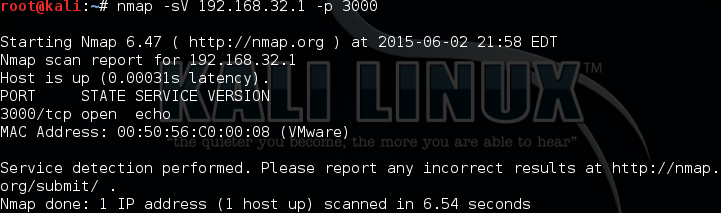
\includegraphics[width=\textwidth]{rsrc/nmap_3}
\caption{Сканирование хост-ОС программой Nmap, из под Kali linux.}
\end{figure}

Nmap распознал, что сервер является эхо-сервисом, но не смог узнать версию сервиса. Попробуем подредактировать файл nmap-service-probes, добавив следующее правило:
\begin{Verbatim}[frame=single]
###########################NEXT PROBE###########################
# Simple TSP server.
Probe TCP simple-tcp-server-ver q|version|
ports 3000
match tcp m|^1.2$| p/Simple TCP Server/ v/1.2/
\end{Verbatim}

Повторное сканирование:

\begin{figure}[h!]
\centering
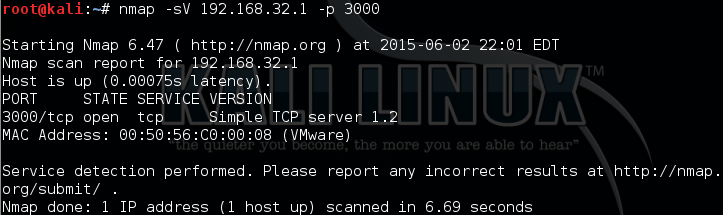
\includegraphics[width=\textwidth]{rsrc/nmap_tcpok}
\caption{Сканирование хост-ОС программой Nmap, из под Kali linux.}
\end{figure}
Версия сервиса определена верно.

\paragraph{Сохранение вывода программы в формате xml\\}
Для сохранения в формате xml используем команду:
\begin{Verbatim}[frame=single]
nmap -sV -p 3000 192.168.32.1 -oX output.xml
\end{Verbatim}

Результат выполнения команды:
\begin{figure}[h!]
\centering
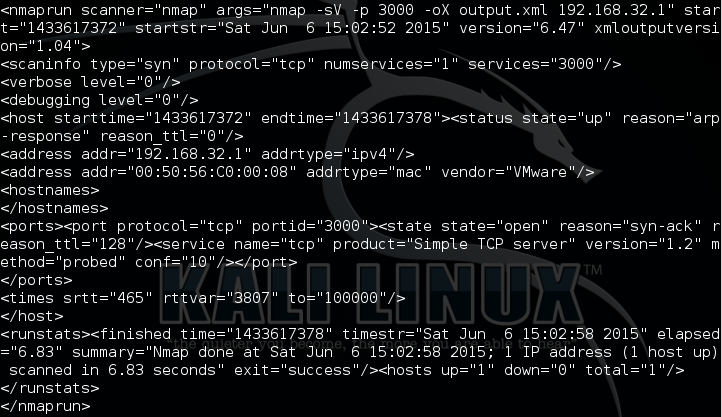
\includegraphics[width=\textwidth]{rsrc/nmap_xml}
\caption{Вывод в .xml формате.}
\end{figure}

\subsubsection{Исследование различных этапов и режимов работы nmap с использованием утилиты Wireshark.}
Функциональность, которую предоставляет Wireshark, очень схожа с возможностями программы tcpdump, однако Wireshark имеет графический пользовательский интерфейс и гораздо больше возможностей по сортировке и фильтрации информации. Программа позволяет пользователю просматривать весь проходящий по сети трафик в режиме реального времени, переводя сетевую карту в неразборчивый режим(promiscuous mode). Программа распространяется под свободной лицензией GNU GPL и использует для формирования графического интерфейса кроссплатформенную библиотеку GTK+. Wireshark — это приложение, которое «знает» структуру самых различных сетевых протоколов, и поэтому позволяет разобрать сетевой пакет, отображая значение каждого поля протокола любого уровня. Поскольку для захвата пакетов используется pcap, существует возможность захвата данных только из тех сетей, которые поддерживаются этой библиотекой.

Для начала работы выберем в списке интерфейс с названием eth0, далее мы будем видеть все пакеты, проходящие через этот интерфейс. Кликаем Start и видим окно, в котором появляются сетевые пакеты по мере их перехвата.Для примера можно послать команду с хост ОС ''ping 192.168.32.130'' - пропинговать Kali linux с основной ОС (адрес 192.168.32.1). Полученные результаты в окне Wireshark:
\begin{figure}[h!]
\centering
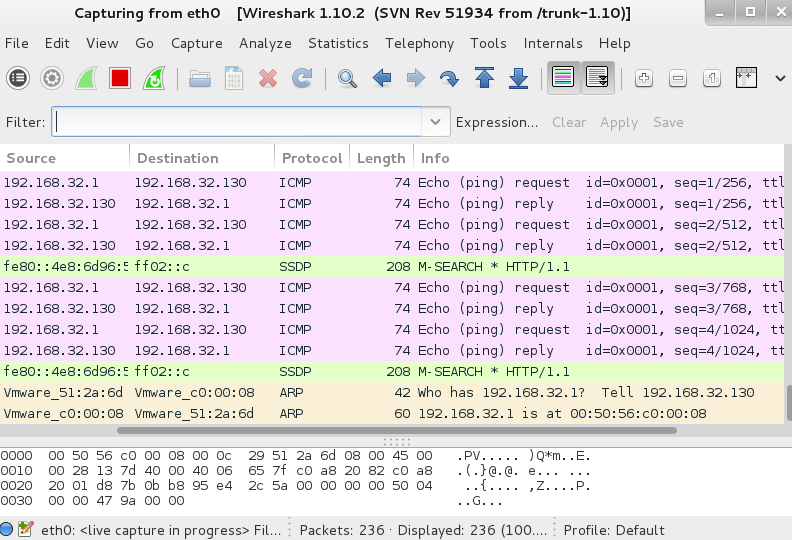
\includegraphics[width=\textwidth]{rsrc/nmap_wireshark_ping}
\caption{Отслеживание ICMP пакетов, используемых командой ping. Видны и четко различимы пакеты, представляющие собой запросы и ответы.}
\end{figure}

Чтобы увидеть работу утилиты nmap в окне wireshark запустим на Kali nmap командой ''nmap -sV -p 3000 192.168.32.1'', а на основной ОС запустим простейший tcp-сервер, использованный ранее. Перед этим запустим прослушивание интерфейса eth0 в wireshark. Применяя в wireshark фильтр по tcp пакетам, получаем последовательность запросов и ответов, инициированных nmap:
\begin{figure}[h!]
\centering
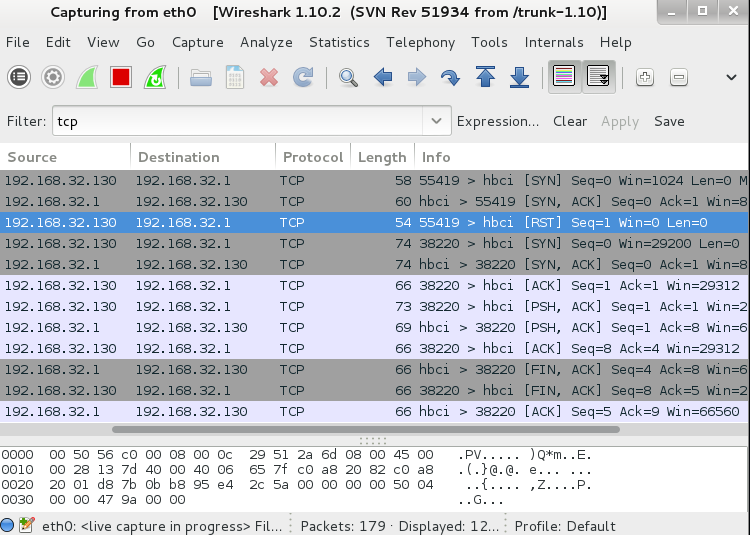
\includegraphics[width=\textwidth]{rsrc/nmap_wireshark_sv}
\caption{Отслеживание tcp пакетов, используемых утилитой nmap. Видны этапы установки соединения, обмена сообщениями и завершения соединения}
\end{figure}

\subsubsection{Сканирование виртуальной машины Metasploitable2 с использованием db\_nmap из состава metasploitframework.}
Обе машины находятся в сети 192.168.32.0/24
\begin{Verbatim}[frame=single]
msf > db_nmap -v -sV 192.168.32.132
[*] Nmap: Starting Nmap 6.47 ( http://nmap.org )
[*] Nmap: NSE: Loaded 29 scripts for scanning.
[*] Nmap: Initiating ARP Ping Scan at 21:05
[*] Nmap: Scanning 192.168.32.132 [1 port]
[*] Nmap: Completed ARP Ping Scan at 21:05, 0.05s elapsed
[*] Nmap: Initiating Parallel DNS resolution of 1 host. at 21:05
[*] Nmap: Completed Parallel DNS resolution of 1 host. at 21:05
[*] Nmap: Initiating SYN Stealth Scan at 21:05
[*] Nmap: Scanning 192.168.32.132 [1000 ports]
[*] Nmap: Discovered open port 22/tcp on 192.168.32.132
[*] Nmap: Discovered open port 5900/tcp on 192.168.32.132
[*] Nmap: Discovered open port 80/tcp on 192.168.32.132
[*] Nmap: Discovered open port 53/tcp on 192.168.32.132
[*] Nmap: Discovered open port 21/tcp on 192.168.32.132
[*] Nmap: Discovered open port 3306/tcp on 192.168.32.132
[*] Nmap: Discovered open port 445/tcp on 192.168.32.132
[*] Nmap: Discovered open port 23/tcp on 192.168.32.132
[*] Nmap: Discovered open port 25/tcp on 192.168.32.132
[*] Nmap: Discovered open port 111/tcp on 192.168.32.132
[*] Nmap: Discovered open port 139/tcp on 192.168.32.132
[*] Nmap: Discovered open port 2049/tcp on 192.168.32.132
[*] Nmap: Discovered open port 512/tcp on 192.168.32.132
[*] Nmap: Discovered open port 8180/tcp on 192.168.32.132
[*] Nmap: Discovered open port 6000/tcp on 192.168.32.132
[*] Nmap: Discovered open port 5432/tcp on 192.168.32.132
[*] Nmap: Discovered open port 1524/tcp on 192.168.32.132
[*] Nmap: Discovered open port 1099/tcp on 192.168.32.132
[*] Nmap: Discovered open port 6667/tcp on 192.168.32.132
[*] Nmap: Discovered open port 514/tcp on 192.168.32.132
[*] Nmap: Discovered open port 2121/tcp on 192.168.32.132
[*] Nmap: Discovered open port 8009/tcp on 192.168.32.132
[*] Nmap: Discovered open port 513/tcp on 192.168.32.132
[*] Nmap: Completed SYN Stealth Scan at 21:05, (1000 ports)
[*] Nmap: Initiating Service scan at 21:05
[*] Nmap: Scanning 23 services on 192.168.32.132
[*] Nmap: Completed Service scan  (23 services on 1  host)
[*] Nmap: NSE: Script scanning 192.168.32.132.
[*] Nmap: Initiating NSE at 21:05
[*] Nmap: Completed NSE at 21:05, 0.16s elapsed
[*] Nmap: Nmap scan report for 192.168.32.132
[*] Nmap: Host is up (0.00030s latency).
[*] Nmap: Not shown: 977 closed ports
[*] Nmap: PORT     STATE SERVICE     VERSION
[*] Nmap: 21/tcp   open  ftp         vsftpd 2.3.4
[*] Nmap: 22/tcp   open  ssh       OpenSSH 4.7p1 Debian 8ubuntu1
[*] Nmap: 23/tcp   open  telnet      Linux telnetd
[*] Nmap: 25/tcp   open  smtp        Postfix smtpd
[*] Nmap: 53/tcp   open  domain      ISC BIND 9.4.2
[*] Nmap: 80/tcp   open  http        Apache httpd 2.2.8
[*] Nmap: 111/tcp  open  rpcbind     2 (RPC #100000)
[*] Nmap: 139/tcp  open  netbios-ssn Samba smbd 3.X
[*] Nmap: 445/tcp  open  netbios-ssn Samba smbd 3.X
[*] Nmap: 512/tcp  open  exec        netkit-rsh rexecd
[*] Nmap: 513/tcp  open  login
[*] Nmap: 514/tcp  open  tcpwrapped
[*] Nmap: 1099/tcp open  rmiregistry GNU Classpath grmiregistry
[*] Nmap: 1524/tcp open  shell       Metasploitable root shell
[*] Nmap: 2049/tcp open  nfs         2-4 (RPC #100003)
[*] Nmap: 2121/tcp open  ftp         ProFTPD 1.3.1
[*] Nmap: 3306/tcp open  mysql       MySQL 5.0.51a-3ubuntu5
[*] Nmap: 5432/tcp open  postgresql  PostgreSQL DB 8.3.0 - 8.3.7
[*] Nmap: 5900/tcp open  vnc         VNC (protocol 3.3)
[*] Nmap: 6000/tcp open  X11         (access denied)
[*] Nmap: 6667/tcp open  irc         Unreal ircd
[*] Nmap: 8009/tcp open  ajp13  Apache Jserv (Protocol v1.3)
[*] Nmap: 8180/tcp open  http  Apache Tomcat
[*] Nmap: MAC Address: 08:00:27:6E:3D:DB (Cadmus Systems)
[*] Nmap: Service Info: Hosts:  metasploitable.localdomain,
 localhost, irc.Metasploitable.LAN; OSs: Unix, Linux; CPE: 
     cpe:/o:linux:linux_kernel
[*] Nmap: Read data files from: /usr/bin/../share/nmap
[*] Nmap: Service detection performed. Please report any
 incorrect results at  http://nmap.org/submit/ .
[*] Nmap: Nmap done: 1 IP address (1 host up)
 scanned in 14.14 seconds
[*] Nmap: Raw packets sent: 1001 (44.028KB) | Rcvd: 1001 (40 KB)
msf > 
\end{Verbatim}


\subsubsection{Выбрать 5 записей из файла nmap-service-probes и описать их работу.}

\paragraph{Запись 1\\}
Предназначена для проверки ответа сервиса на пустую строку. Предполагается ответ в течении 6 секунд, если ответа не последовало, то выполняется следующий тест.
\begin{figure}[h!]
\centering
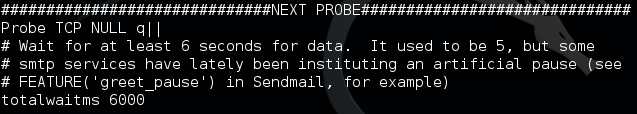
\includegraphics[width=\textwidth]{rsrc/nmap_entry1}
\caption{Запись 1''.}
\end{figure}

\paragraph{Запись 2\\}
Запись проверяет сервис на соответствие протооколу FTP и ожидает что это программа FileZilla.
\begin{figure}[h!]
\centering
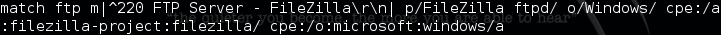
\includegraphics[width=\textwidth]{rsrc/nmap_entry2}
\caption{Запись 2''.}
\end{figure}

\paragraph{Запись 3\\}
Запись проверяет, что на запрос отвечает служба gkrellm. Ожидает одну из двух ошибок (либо обе, поскольку поставлено правило \textbf{softmatch}, а не \textbf{match} и по нему тестирование не переходит к следующему тесту при ошибке, а продолжает текущий тест).
\begin{figure}[h!]
\centering
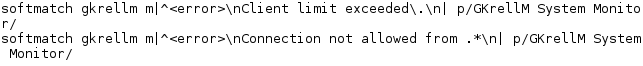
\includegraphics[width=\textwidth]{rsrc/nmap_entry3}
\caption{Запись 3''.}
\end{figure}

\paragraph{Запись 4\\}
Запись тестирует сервис на принадлежность протоколу pop3. Ожидается ответ ''+ОК AppleMailServer ...''. Вероятнее всего, что ожидается, что сервисом является какой-либо почтовый сервер от компании Apple.
\begin{figure}[h!]
\centering
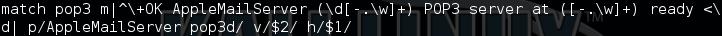
\includegraphics[width=\textwidth]{rsrc/nmap_entry4}
\caption{Запись 4''.}
\end{figure}

\paragraph{Запись 5\\}
Запись тестирует сервис на принадлежность протоколу http. Предполагается,что сервисом является Microsoft IIS Server - http сервер от Microsoft. Правило предполагает возвращение http-кода 400, что соответствует 400 Bad Request — сервер обнаружил в запросе клиента синтаксическую ошибку.
\begin{figure}[h!]
\centering
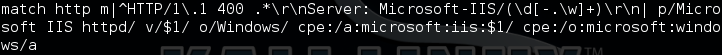
\includegraphics[width=\textwidth]{rsrc/nmap_entry5}
\caption{Запись 5'.}
\end{figure}

\newpage
\subsubsection{Выбрать один скрипт из состава Nmap и описать его работу.}

Выберем скрипт под именем ftp-anon.nse. Этот скрипт предназначен для проверки FTP-сервера на возможность анонимного подключения. Скрипт посылает команду PASV и ждет порт для подключения. Затем он запрашивает список директорий командой LIST и ожидает ответ в формате что-то вроде ''2хх Entering Passive Mode ... ''. Если сервер вернул код 332, то есть нужен аккаунт для логина, то анонимные подключения на сервере запрещены.
Для запуска скрипта используем команду:
\begin{Verbatim}[frame=single]
nmap --script ''ftp-anon.nse'' 151.80.164.83
\end{Verbatim}
Полученные результаты:
\begin{figure}[h!]
\centering
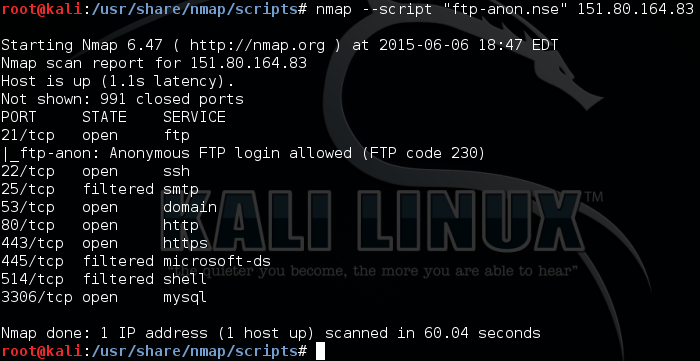
\includegraphics[width=\textwidth]{rsrc/nmap_nse_ftp}
\caption{Сканирование FTP-сервера программой Nmap с использованием скрипта ''ftp-anon.nse''.}
\end{figure}


\subsection{Выводы}
nmap — свободная утилита, предназначенная для разнообразного настраиваемого сканирования IP-сетей с любым количеством объектов, определения состояния объектов сканируемой сети (портов и соответствующих им служб). Nmap использует множество различных методов сканирования, таких как UDP, TCP (connect), TCP SYN (полуоткрытое), FTP-proxy (прорыв через ftp), Reverse-ident, ICMP (ping), FIN, ACK, Xmas tree, SYN- и NULL-сканирование. Использование nmap позволяет находить потенциальные уязвимости в сетевых сервисах хостов. Это может помочь системному администратору закрыть уязвимости в безопасности сети и повысить уровень ее надежности.



\end{document}